\subsection{Simulaciones}
\label{subsec:simulaciones}

En esta sección, se describe el proceso de creación del modelo de la lanzadera electromagnética realizado utilizando ANSYS Maxwell. Este software de métodos finitos está especializado en el análisis de sistemas electromagnéticos. El objetivo de estas simulaciones es obtener una comprensión detallada del comportamiento del campo magnético generado por la bobina y su interacción con el proyectil ferromagnético en la lanzadera electromagnética. Se ha dividido el proceso en tres subapartados: creación de la geometría, simulaciones instantáneas y simulaciones transitorias. En la primera, se mostrará el proceso de creación de la geometría paramétrica en 2D y 3D, en la segunda y tercera se explicarán las condiciones de contorno y resultados de las simulaciones instantáneas y transitorias, respectivamente.

\subsubsection{Geometría}
El primer paso para realizar las simulaciones fue la creación de la geometría del sistema en ANSYS Maxwell. Para ello, se definieron las dimensiones y características de la bobina y el proyectil de manera paramétrica. Esto quiere decir que las dimensiones de los polígonos que conforman el modelo no son fijas, si no que están asociados a variables por lo que simular diferentes configuraciones se convierte en algo más sencillo. La geometría fue primeramente diseñada en 3D, pero también se obtuvo la sección central del archivo tridimensional para poder simular en 2D, lo que a priori permite menor tiempo de computación. Una vez creada la geometría, se definieron los diferentes materiales y las propiedades eléctricas y magnéticas. El material utilizado para los conductores del solenoide es cobre recocido, PVC para el soporte de la bobina y \textbf{FALTA EL ACERO} para el vástago. Con esto, se construye la geometría a continuación mostrada:

\begin{itemize}
    \item \textbf{Geometría en 3D}:
    %insertar geom 3D
    \item \textbf{Mallado en 3D}:
    %insertar mallado 3D
    \item \textbf{Geometría en 2D}:
    \begin{figure}[H]
        \centering
        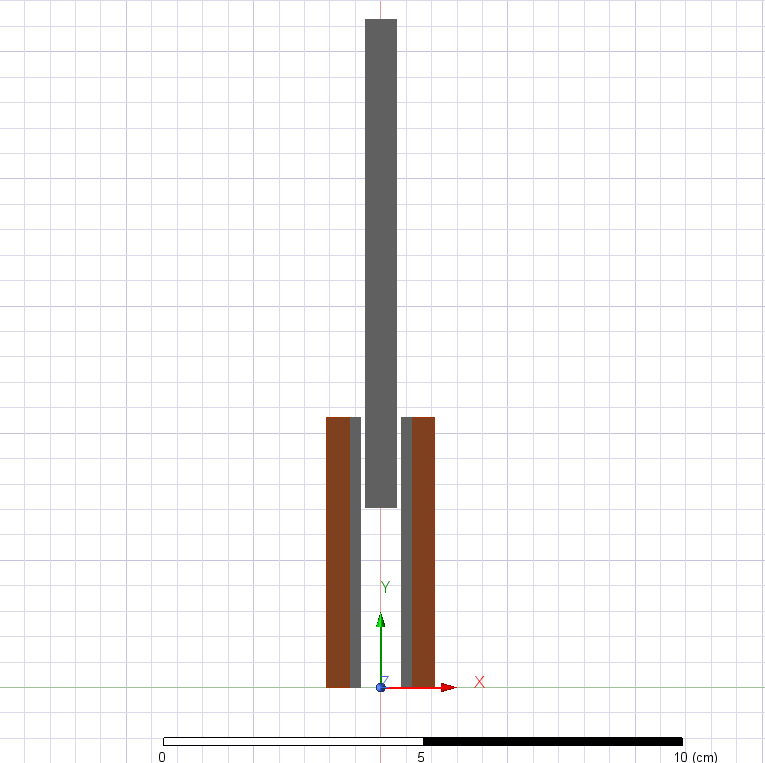
\includegraphics[width=9cm]{FigurasMemoria/BarGeom.png}
        \caption{Geometría de la barra y bobina en 2D. Elaboración propia.}
        \label{fig:BarGeom} %Para referenciar -> \ref{fig:figNum}
    \end{figure}
    \item \textbf{Mallado en 2D}
    \begin{figure}[H]
        \centering
        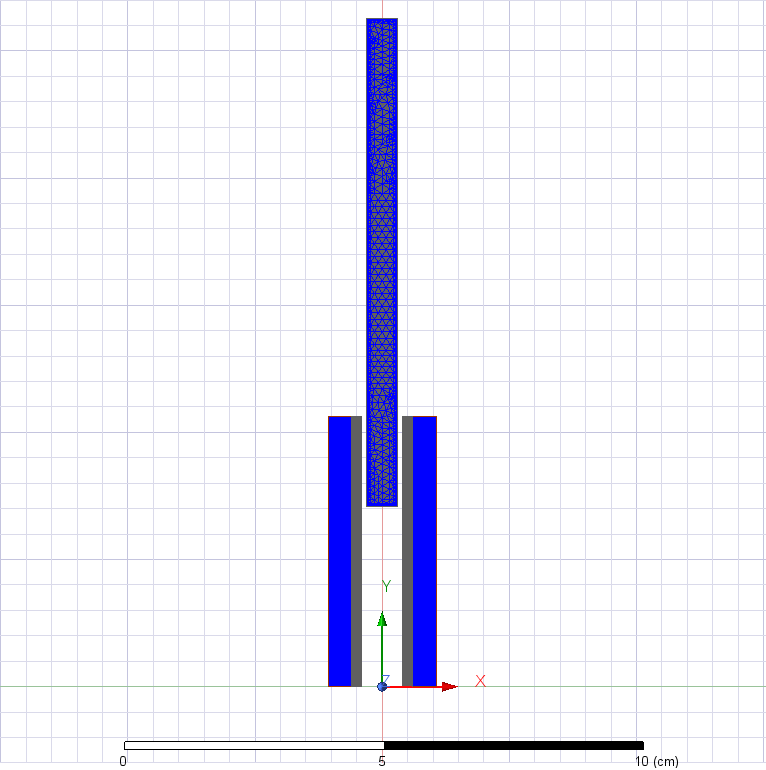
\includegraphics[width=9cm]{FigurasMemoria/BarGeomMesh.png}
        \caption{Mallado de la barra y bobina en 2D. Elaboración propia.}
        \label{fig:BarGeomMesh} %Para referenciar -> \ref{fig:figNum}
    \end{figure}
    \begin{figure}[H]
        \centering
        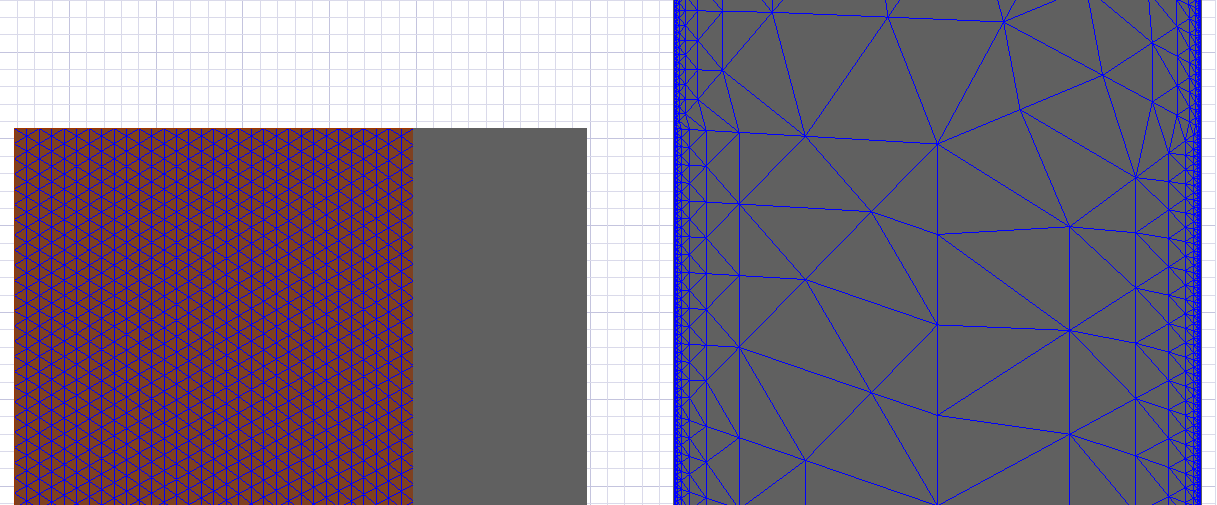
\includegraphics[width=9cm]{FigurasMemoria/BarMeshDetail.png}
        \caption{Detalle del mallado de la barra y bobina en 2D. Elaboración propia.}
        \label{fig:GeomMeshDetail} %Para referenciar -> \ref{fig:figNum}
    \end{figure}
\end{itemize}

La bobina se ha generado de la forma mostrada en las figuras anteriores debido a que representar un número de espiras del orden de \(10^2\) de manera helicoidal y con varias capas es muy complicado en ANSYS, ya que no es un entorno de diseño en 3D. Al crear un cilindro con dimensiones apropiadas, se puede indicar al software que lo trate como un solenoide, asignándole un número de espiras y una corriente de excitación. El programa distribuye uniformemente el campo generado por la corriente en todo el volumen, lo que resulta en una aproximación muy válida \citep[p. 13]{ansoft2012maxwell}.

\subsubsection{Simulaciones instantáneas}
ANSYS Maxwell permite realizar simulaciones de diferentes tipos, de las cuales tienen interés para este proyecto las magnetoestáticas y las transitorias. Como primera prueba para el modelo de la figura \textbf{FIGURA3D}, se realizó una simulación electroestática con una \(I_{cc}=3.5~A\) para poder observar los campos magnéticos del sistema, resultando en la siguiente figura:

\begin{figure}[H]
    \centering
    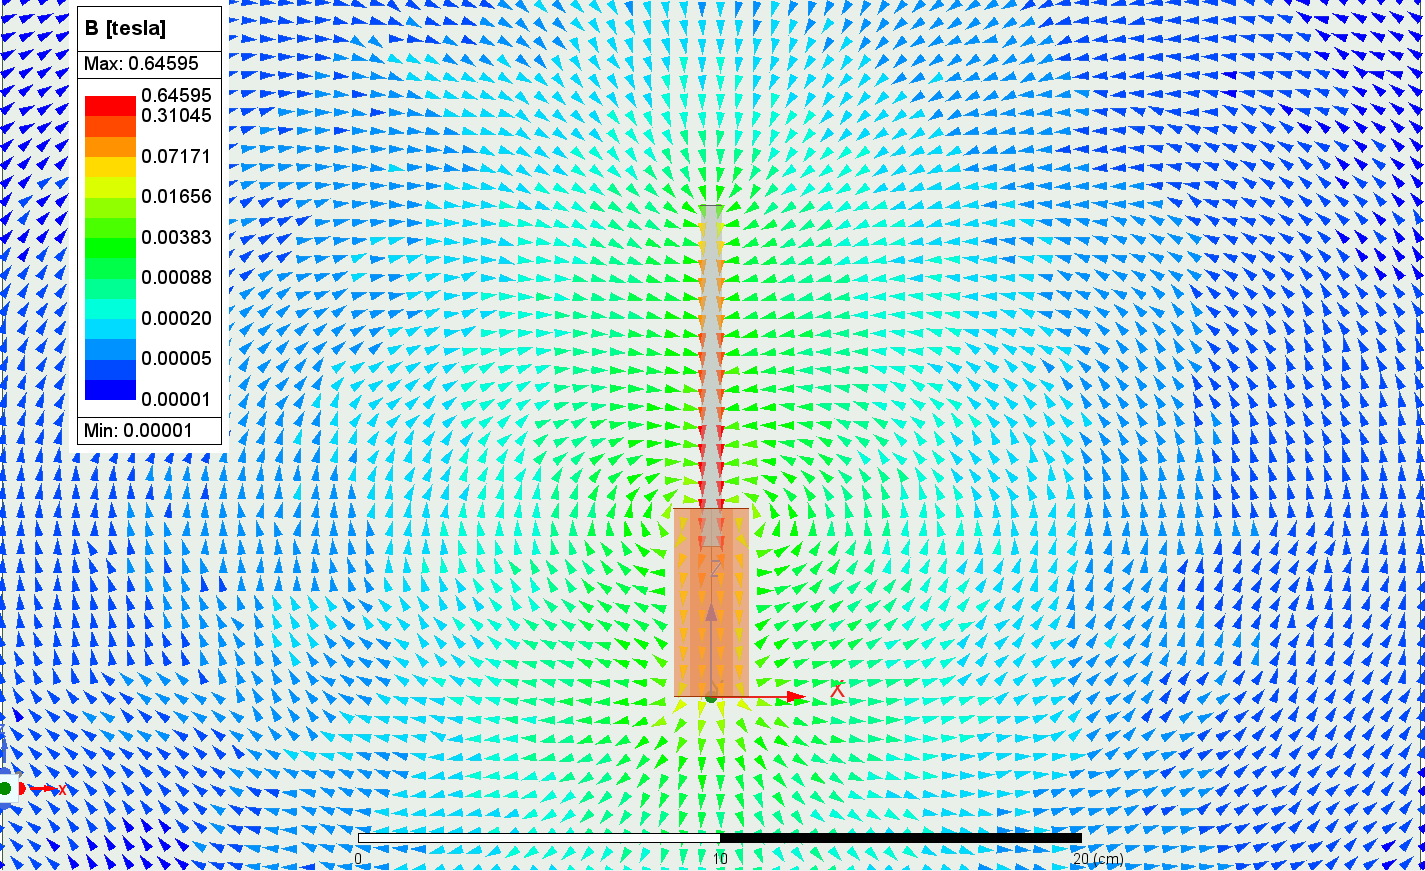
\includegraphics[width=\linewidth]{FigurasMemoria/fields8.PNG}
    \caption{Visualización de los campos magnéticos con la bobina energizada y \(x=2/10 * h_c\). Elaboración propia.}
    \label{fig:fields8} %Para referenciar -> \ref{fig:figNum}
\end{figure}

Vemos que se puede apreciar perfectamente la forma descrita en las figuras \ref{fig:integralampere} y \ref{fig:electromagnet}, curvándose en los extremos del sistema pero permaneciendo bastante uniforme a lo largo de \(h_c\). Se muestra a continuación un detalle de los campos únicamente dentro de la bobina con la barra en la posición de la figura \ref{fig:fields8}:

\begin{figure}[H]
    \centering
    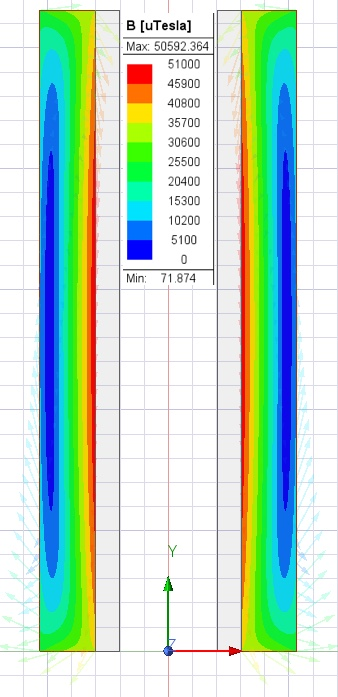
\includegraphics[width=4cm]{FigurasMemoria/fieldsDetail.jpg}
    \caption{Visualización de los campos magnéticos dentro del solenoide. Elaboración propia.}
    \label{fig:fieldsDetail} %Para referenciar -> \ref{fig:figNum}
\end{figure}

Además de visualizar los campos, ANSYS Maxwell permite añadir distintas medidas a la simulación, entre las que se encuentra la fuerza de atracción magnética. Realizando la simulación de nuevo para la configuración en 3D, se obtiene que la fuerza es igual a:

\begin{table}[h]
    \centering
    \begin{tabular}{|c|c|c|c|c|}
        \hline
        & \(F_x\) & \(F_y\) & \(F_z\) & \(F_{tot}\) \\
        \hline
        \(F_{ANSYS}\) & Data 2 & Data 3 & Data 4 & Data 5 \\
        \hline
    \end{tabular}
    \caption{Fuerzas de atracción magnética en los diferentes ejes del espacio. Elaboración propia.}
    \label{tab:fuerzas}
\end{table}
